%% Refer elsdoc for options available for "Document Class"
\documentclass[preprint]{elsarticle}

%% \usepackage{lineno}
\usepackage{lineno,hyperref}
% if you have landscape tables
\usepackage[figuresright]{rotating}

%% Custom Packages
\usepackage{float} %% For image placement

%% Put line numbers for every line.
\modulolinenumbers[1] 

%% Enter Journal Name here
\journal{Materials and Design}
%%%%%%%%%%%%%%%%%%%%%%%%%%%%%%%%%%%%%%%%%%%%%%%%%%%%%%%%%%%%%%%%%%%%%%%%%%

%% The amssymb package provides various useful mathematical symbols
%%\usepackage{amssymb}
%% The amsthm package provides extended theorem environments
%% \usepackage{amsthm}

%%%%%%%%%%%%%%%%%%%%%%%
%% Reference Styling %%
%%%%%%%%%%%%%%%%%%%%%%%

%% natbib.sty is loaded by default. However, natbib options can be
%% provided with \biboptions{...} command. Following options are
%% valid:

%%   round  -  round parentheses are used (default)
%%   square -  square brackets are used   [option]
%%   curly  -  curly braces are used      {option}
%%   angle  -  angle brackets are used    <option>
%%   semicolon  -  multiple citations separated by semi-colon
%%   colon  - same as semicolon, an earlier confusion
%%   comma  -  separated by comma
%%   numbers-  selects numerical citations
%%   super  -  numerical citations as superscripts
%%   sort   -  sorts multiple citations according to order in ref. list
%%   sort&compress   -  like sort, but also compresses numerical citations
%%   compress - compresses without sorting
%%
%% Example : \biboptions{comma,round}

\biboptions{square,comma,sort&compress}
%%%%%%%%%%%%%%%%%%%%%%%%%%%%%%%%%%%%%%%%%%%%%%%%%%%%%%%%%%%%%%%%%%%%%%%%%%
                   %% Declarations for front matter
\begin{document}
                   %% Declarations of Commands
\newcommand{\degree}[1]{\ensuremath{^{\circ}}}  %% Command for degree



\begin{frontmatter}

\title{Friction welding of Ti-6Al-4V tube to AA6061 tube-plate using an external tool}

%%%%%%%%%%%%%%%%%%%%%%%%%%%%%%%%%%%%%%%%%%%%%%%%%%%%%%%%%%%%%%%%%%%%%%%%%%
                      %% Author Declaration
\author[META]{Sharan. C}
\ead{Sharanc25@gmail.com}
\author[META]{Maxwell Rejil. C}
\ead{maxwellrejilc@gmail.com}
\author[META]{Sooraj. R}
\ead{soorajramana89@gmail.com}
\author[META]{Muthukumaran. S\corref{cor1}}
\ead{smuthu@nitt.edu}
%\ead[url]{http://www.nitt.edu/home/academics/departments/meta/faculty/asstprof/smuthu}

\cortext[cor1]{Corresponding Author}

\address[META]{Department of Metallurgical and Materials Engineering, National Institute of Technology, Tiruchirappalli-620015, India}
%%%%%%%%%%%%%%%%%%%%%%%%%%%%%%%%%%%%%%%%%%%%%%%%%%%%%%%%%%%%%%%%%%%%%%%%%%
         
\begin{abstract}
Using a new patented process - Friction welding of tube to tube plate using an external tool (FWTPET), Ti-6Al-4V tube and AA6061-T651 tube plate were welded together. The welding was carried out at 4 different speeds with two different tube profiles (Holes and Petals). The effect of tube profile on the joint strength of the welded samples was measured using an in-house developed test procedure named ``Plunge Shear Test''. Fractography studies were carried out on the  sheared surfaces. SEM and XRD analysis was done at the joint interface to study the effect of intermetallics on the joint strength.
\end{abstract}

\begin{keyword}
Ti-6Al-4V \sep AA6062 \sep FWTPET \sep Plunge Shear Test \sep TiAl
\end{keyword}

\end{frontmatter}

%%%%%%%%%%%%%%%%%%%%%%%%%%%%%%%%%%%%%%%%%%%%%%%%%%%%%%%%%%%%%%%%%%%%%%%%%%
							 %%Line Numbers
%% Start line numbering with
%% \begin{linenumbers}, end it with \end{linenumbers}. Or switch it on
%% for the whole article with \linenumbers after \end{frontmatter}.

\linenumbers
%%%%%%%%%%%%%%%%%%%%%%%%%%%%%%%%%%%%%%%%%%%%%%%%%%%%%%%%%%%%%%%%%%%%%%%%%%
							  %%Sections
								
\section{Introduction}
\label{sec:Introduction}
Friction welding of tube to tube plate using an external tool (FWTPET) is a new solid state welding process, invented and patented by Dr. S. Muthukumaran in the year 2006. This process uses an external tool which has a shoulder and a pin. FWTPET process can be carried out in two methods - interference and clearance. Unlike FSW process, in FWTPET the tool pin acts as an anvil and does not cause any stirring action\cite{SenthilKumaran2011}. The parameters that affect the joint strength of a FWTPET welded joints are : tool rotational speed, tube profile, tool shoulder and pin dimension, heat input etc. Our aim was to increase the heat input study its effect of on joint strength. In order to increase the heat input we needed to increase the tool shoulder and tube contact area. 
Although FWTPET is a solid state welding process, in our study, during welding the temperature exceeded the melting point of the aluminium alloy. Thus our current study is a quasi-solid state welding process. 
\par 
AA6061 is a low melting soft metal whereas Ti-6Al-4V is a high melting hard material. The only similarity between these two metals is that both are light weight alloys. Welding a low melting alloy (AA6061) with a high temperature material (Ti-6Al-4V) is extremely difficult by conventional fusion welding process. This leads to lesser heat generation at interface and in turn leads to lesser intermetallic formation when compared to Friction Stir Welding (FSW) processes \cite{MadhusudhanReddy2009}.

%%%%%%%%%%%%%%%%%%%%%%%%%%%%%%%%%%%%%%%%%%Experimental Details%%%%%%%%%%%%%%%%%%%%%%%%%%%%%%%%%%%%%%

\section{Experimental Details} 
\label{sec:Experimental Details}
\subsection{Materials}
\label{subsec:Materials}
AA6061 plates of 6 mm thickness and Titanium Grade V (Ti-6Al-4V) tubes of 19 mm outer diameter were used for welding. The base material composition of AA6061 is given in Table~\ref{table:AA6061-composition} and Ti-6Al-4V is given in Table~\ref{table:Ti-6Al-4V-composition}. The external tool used for welding was made of Tungsten alloy (Figure~\ref{fig:tool}) having 29mm shoulder diameter and 12.5mm pin diameter. Chemical composition of the external tool is given in Table~\ref{table:tool-composition}. 

\begin{table}[!htbp]
\caption{CHEMICAL COMPOSITION OF Ti-6Al-4V}
\centering
\begin{tabular}{|c|c|c|c|c|c|c|c|c|c|}
\hline 
Element & C & Fe & O & N & Al & H & V & Y & Ti\\ 
\hline 
Wt \% & 0.08 & 0.03 & 0.2 & 0.05 & 0.148 & 5.5-6.75 & 3.5-4.5 & 0.005 & balance\\ 
\hline 
\end{tabular}
\label{table:Ti-6Al-4V-composition} % is used to refer this table in the text
\end{table}


\begin{table*}[!htbp]
\caption{CHEMICAL COMPOSITION OF AA6061}
\centering
\begin{tabular}{|c|c|c|c|c|c|c|c|c|c|}
\hline 
Element & Mg & Si & Fe & Cu & Cr & Mn & Ti & Zn & Al\\ 
\hline 
Wt \% & 0.70 & 0.43 & 0.497 & 0.164 & 0.148 & 0.045 & 0.0495 & 0.0042 & balance\\ 
\hline 
\end{tabular}
\label{table:AA6061-composition} % is used to refer this table in the text
\end{table*}

\begin{table*}[!htbp]
\caption{CHEMICAL COMPOSITION OF TOOL MATERIAL}
\centering
\begin{tabular}{|c|c|c|c|c|c|}
\hline 
Element & W & Ni & Co & Fe & O \\ 
\hline 
Wt \% & 90.5 & 5.3 & 0.2 & 3.4 & 0.007 \\ 
\hline 
\end{tabular}
\label{table:tool-composition} % is used to refer this table in the text
\end{table*}

\begin{figure}[H]
\centering
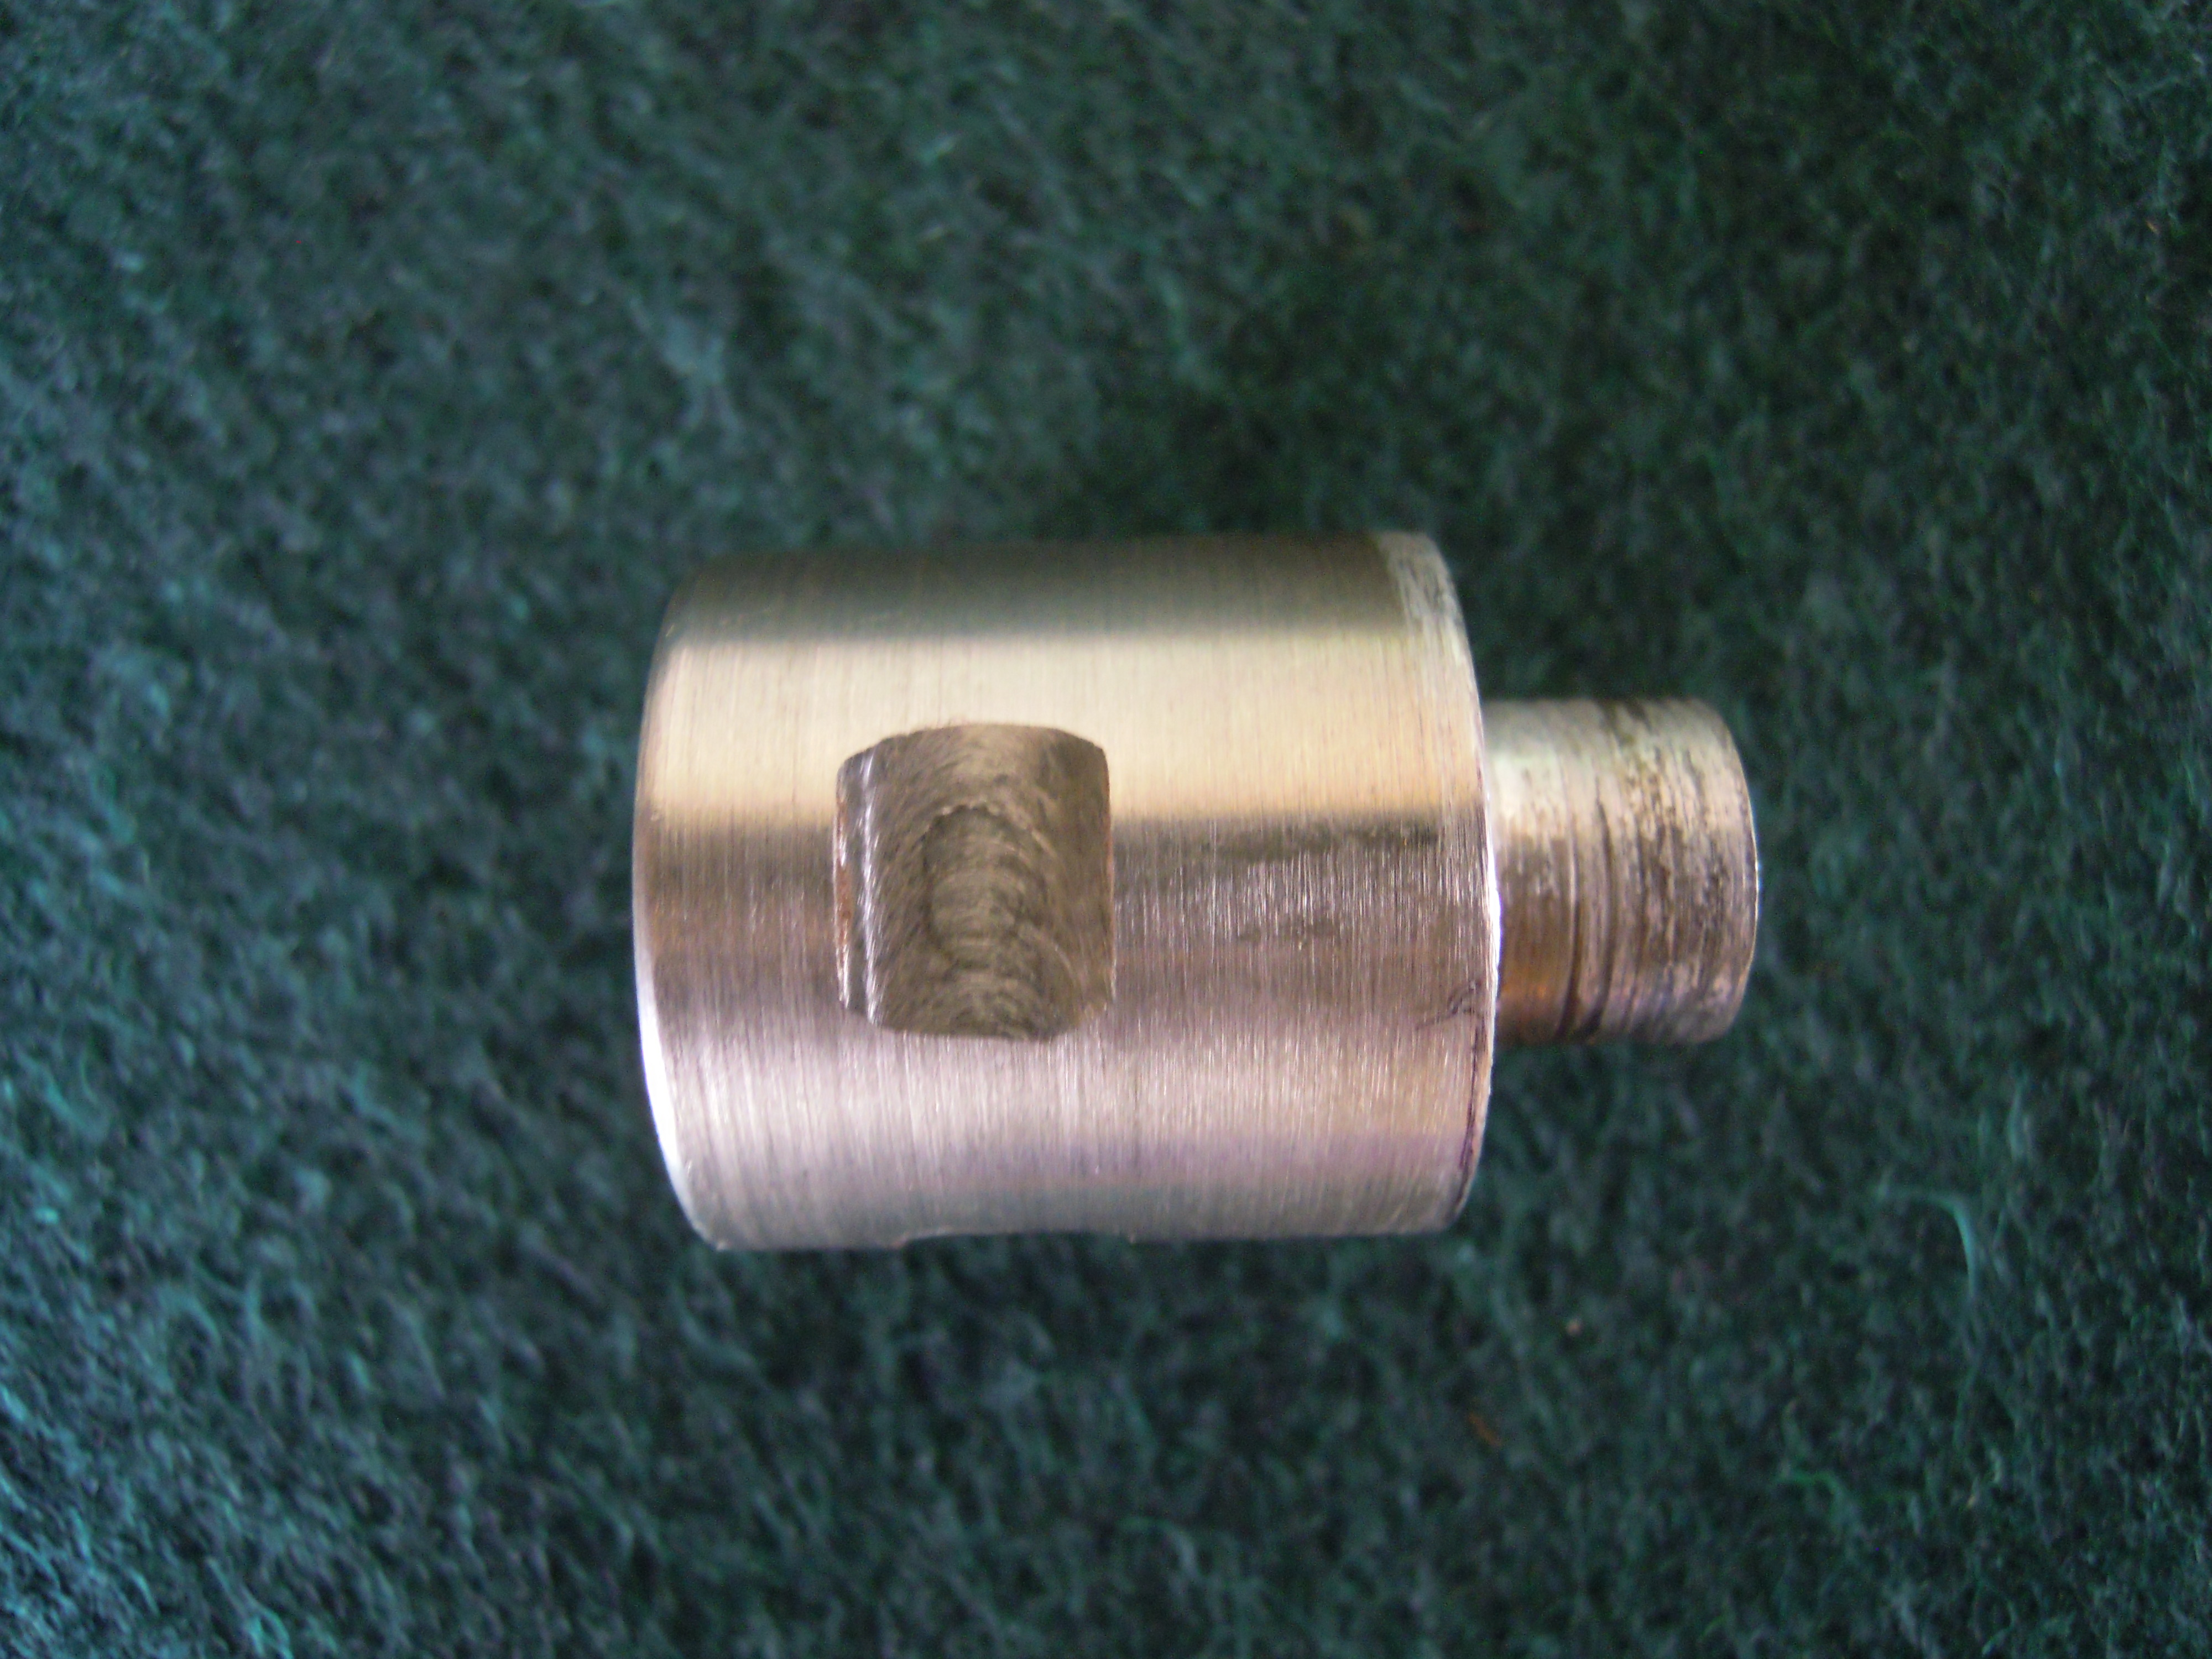
\includegraphics[width=\textwidth]{images/Tool.jpg}
\caption{Tungsten Heavy Alloy Tool}
\label{fig:tool}
\end{figure}

\subsection{FWTPET}
\label{subsec:FWTPET}
FWTPET was carried out in a 4-Axis Friction Stir Welding machine (Fig. 3). For welding, AA6061 plates of 50 x 50 x 6 mm with a hole of 19 mm diameter at the center was used. Ti-6Al-4V tube of 19 mm outer diameter and 14 mm inner diameter and 20 mm length was used for welding. Before welding, both the tube and plate were cleaned with Acetone to remove grease, dirt etc. The tube and plate were fitted to a custom-made backing block as shown in Fig. 3. The parameters used for welding were – tool rotational speed - 1120 rpm, plunge rate – 2 mm/min, plunge depth - 2 mm. These parameters were kept constant for all subsequent welds.

\subsection{Plunge Shear Test}
\label{subsec:Plunge Shear Test}
Due to lack of standard testing procedure to measure the joint strength of tube to tube plate joints, we developed a new testing procedure called ``Plunge Shear Test''. Plunge Shear Test (PST) is a destructive testing method which can be carried out in a conventional Universal testing Machine with the help of an external plunger. To perform the PST, a specially designed tube must be used for welding. For our welding process, a rod of 19 mm diameter and 35mm length was taken and a hole of 14mm diameter was drilled upto a depth of 20 mm as shown in Fig. With the help of a plunger (Fig. 4), a compressive load was applied on the inner diameter of the tube in an UTM until the joint breaks. Using the fracture load obtained, we then calculate the weld strength. Weld strength is calculated by dividing the Fracture load by the weld area.

\subsection{Characterization}
\label{subsec:Characterization}
The welded samples were sectioned at the weld joint to study the microstructural properties. Studies were made using a standard stereoscope and optical microscope. SEM and EDS analysis were performed to quantify the elemental weight percentage at the joint interface. The observations were carried out in a 200kV field effect scanning electron microscope (SEM-JEOL JSM 5410LV microscopy) coupled with EDS. EDS line scan was also carried out along the weld interface. XRD analysis was done at the weld interface of Al-Ti dissimilar welds. XRD analysis helps to find out the formation of intermetallic at the weld interface. Scan speed was 10º/min and step width was 0.02º. In order to reveal the microstructures, AA6061-T651 plate specimens were etched with Poulton’s reagent (30ml HCl, 40ml HNO3, 2.5 mL HF, 12 g CrO3, 42.5 mL H2O). The etchant time used was 10-15 seconds. Ti-6Al-4V tube specimens were etched with Kroll’s reagent (192ml H2O, 5mL HNO3, 3ml HCl, 2ml HF) for 25-30 seconds. Microstructures and macrostructures were taken using an optical microscope.


%%%%%%%%%%%%%%%%%%%%%%%%%%%%%%%%%%%%%%%%%%Results and Discussion%%%%%%%%%%%%%%%%%%%%%%%%%%%%%%%%%%%%%%
\section{Results and Discussion}
\label{sec:Results and Discussion}

\subsection{Macrostructure Analysis}
\label{subsec:Macrostructure Analysis}
The macrostructures, for all three different tube profiles revealed defect free joints. For tube with holes profile, Aluminium is embedded in the Titanium region (Fig. 5 a,b). Plates welded with tube having petals are characterized by Titanium deposited on the surface of the Aluminium plates (Fig. 5 c).

\subsection{Microstructure Analysis}
\label{subsec:Macrostructure Analysis}
The microstructure of AA6061-T651 base metal is shown in Fig. 6. Optical micrographs of the base AA6061-T6 revealed the presence of Mg2Si precipitates which strengthens the Al alloy [4]. Ti-6Al-4V is an α-β alloy that has a “Basket Weave” microstructure in which retained β lies between α platelets in a Widmanstӓtten structure, itself contains thinner secondary α platelets [5]. In Fig. 7, the dark lines in the microstructure are
the β phase and the light region is α phase.

\subsection{Weld Strength}
\label{subsec:Weld Strength}
Weld strength was measured by using the shear fracture load obtained from PST. Shearing will take place along the interface of the welded sample. The shear strength values for different tube profiles are given in Table II. From the table, it is clear that tube with petals is having high shear strength compared to other to profiles. This is due to the increase in weld area when compared to other tube profiles.

\subsection{X-Ray Diffraction Analysis}
\label{subsec:XRD-Results}
XRD plot at the weld interface for welds made with Tube with petals is shown in Fig. 12. From the XRD plot, the
presence of TiAl3 intermetallic formation was observed. Formation of intermetallic compounds is detrimental to joint strength. Titanium aluminide has three major intermetallic compounds: γ TiAl, α Ti3Al and TiAl3. Although these intermetallics have very good mechanical and thermal properties, they have very low ductility [6]. Therefore, the presence of Titanium aluminides at the interface might decrease the joint strength.

\subsection{SEM Analysis}
\label{subsec:SEM Analysis}
SEM micrograph (Fig. 13) shows the Titanium particles entirely entrapped in the Al matrix at the weld interface. It can be seen that thick mixed layers are formed on the interface. EDS Line Scanning analysis was done along the interface. EDS patterns and element contents are shown in Fig. 14.

\subsection{Fractography}
\label{subsec:Fractography}
The SEM image (Fig. 15) shows fracture surface of Titanium tube for petal profile after the PST. From the image, we can clearly see some areas on the fracture surface where the aluminum alloy is still bonded to Titanium. SEM images of the fracture surface on the Aluminum plate shows cleavage facets, which is an indication shear fracture [7],[8]. Some Titanium particles embedded in the Aluminium matrix are also visible in
the SEM images (Fig. 16 b).

\section{Conclusion}
\label{sec:Conclusion}
\begin{enumerate}[1.]
\item FWTPET method has been established to join 6mm thick Aluminum (AA6061-T651) tube plate to Titanium (Ti-6Al-4V) tubes of 2.5mm wall thickness.
\item Three different tube profiles-hole, slot and petals, were used to study the feasibility of joining dissimilar materials (Al-Ti) using FWTPET and petal profile was found to have good strength.
\item Shear strength of the joint reached 60% of AA6061–T651 base material strength.
\item XRD analysis showed formation of TiAl3 at the interface. Intermetallic compounds at the interface were less when compared to traditional fusion welding processes which is due to the reduction in heat generation during the welding process.
\end{enumerate}

%%%%%%%%%%%%%%%%%%%%%%%%%%%%%%%%%%%%%%%%%%%%%%%%%%%%%%%%%%%%%%%%%%%%%%%%%%
							%%References
%% Following citation commands can be used in the body text:
%% Usage of \cite is as follows:
%%   \cite{key}         ==>>  [#]
%%   \cite[chap. 2]{key} ==>> [#, chap. 2]
%%

%%%%%%%%%%%%%%%%%%%%%%%%%%%%%%%%%%
%% Elsevier bibliography styles %%
%%%%%%%%%%%%%%%%%%%%%%%%%%%%%%%%%%
%% Numbered
%\bibliographystyle{model1-num-names}

%% Numbered without titles
%\bibliographystyle{model1a-num-names}

%% Harvard
%\bibliographystyle{model2-names.bst}\biboptions{authoryear}

%% Vancouver numbered
%\usepackage{numcompress}\bibliographystyle{model3-num-names}

%% Vancouver name/year
%\usepackage{numcompress}\bibliographystyle{model4-names}\biboptions{authoryear}

%% APA style
%\bibliographystyle{model5-names}\biboptions{authoryear}

%% AMA style
%\usepackage{numcompress}\bibliographystyle{model6-num-names}

%% `Elsevier LaTeX' style
\bibliographystyle{elsarticle-num}

%% References with BibTeX database:
%% Authors are advised to use a BibTeX database file for their reference list.
%% The provided style file elsarticle-num.bst formats references in the required style

\bibliography{bibtex-database}

%% For references without a BibTeX database:

% \begin{thebibliography}{00}

%% \bibitem must have the following form:
%%   \bibitem{key}...
%%

% \bibitem{}

% \end{thebibliography}
%%%%%%%%%%%%%%%%%%%%%%%%%%%%%%%%%%%%%%%%%%%%%%%%%%%%%%%%%%%%%%%%%%%%%%%%%%
							%%Appendix
%% The Appendices part is started with the command \appendix;
%% appendix sections are then done as normal sections
%% \appendix

\end{document}